
\begin{document}

\chapter{Results}

\label{chapter:results}

This chapter presents the results from the experimentation of the algorithm.
The metrics used and the experimental setup is described in
Ch.~\ref{chapter:experimentalsetup}. This chapter will describe the empirical
data gathered for the safety and computational time of the algorithm developed
in Sec.~\ref{sec:design_planner}. This chapter will also compare the proposed
approach with a more standard approach, potential fields, using the empirical
data gathered. For all of the plots presented, the data for the algorithm
developed in this work is shown on the left and the data for the standard
potential fields planner is shown on the right. Also note that this chapter
only surveys the results for Scene 1 because the data was very similar for all
of the scenes. The plots for the other scenes is shown in the appendix.

\section{Safety}

Providing an empirical evaluation of the safety of the developed planner is
incredibly important because if it does not provide quantifiable safe paths
through the environment, the main objective was not satisfied. This section
presents the data gathered for the three safety metrics with the experimental
setup described in Ch.~\ref{chapter:experimentalsetup}. The three safety
metrics are the minimum distance at any given time during the execution of the
path to a dynamic obstacle, the maximum cost along the path given by the cost
distribution discussed in Eq.~\ref{eq:cost}, and the average cost along the
path.

Fig.~\ref{fig:plot_min_distance} shows how the mean minimum distance changes as
a function of the set speed of the robot and the amount of noise introduced to
the trajectories of obstacles. The larger the minimum distance, the safer the
path is. From the figure, it is evident that as the speed increases, so does
the mean minimum distance Dodger. The amount of noise injected into the
obstacle trajectories, $\epsilon$, does not seem to have any major effect on
the minimum distance for any speed. For potential fields, as the speed
increases, the increase in the minimum distance is not as drastic and the noise
does not affect the overall safety given this metric. The differences between
these two plots stem from the fact that a potential fields planner is purely
reactive and Dodger generates a path by looking ahead. This means that the
potential fields planner could move the robot through the path of an obstacle
thus decreasing the minimum distance and increasing the possibility of a
collision. Dodger will avoid moving the robot through the trajectory of an
obstacle and thus is more likely to have a larger minimum distance along the
path. For the gathered empirical data shown in
Fig.~\ref{fig:plot_min_distance}, Dodger provided paths with a higher overall
minimum distance than potential fields and as the speed of the robot increased,
the minimum distance for the paths generated by Dodger out performed those
generated by potential fields for this metric.

\begin{figure}[h!]
    \centering
    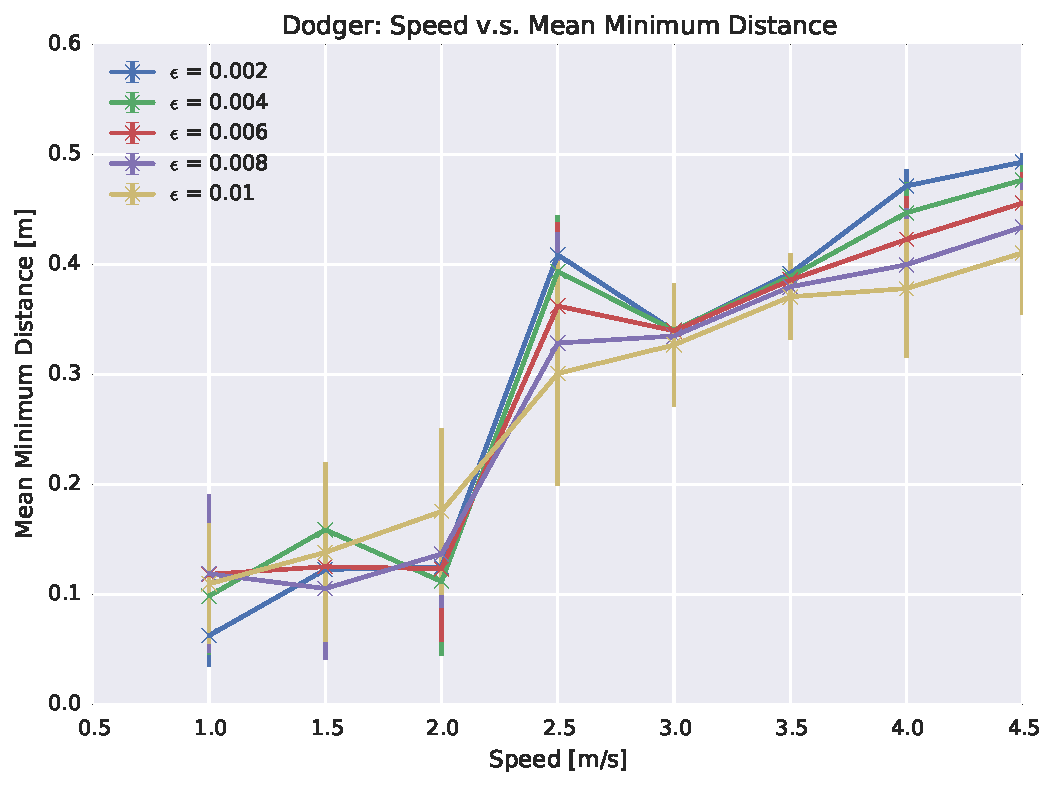
\includegraphics[width=0.48\linewidth]{figs/planner_mean_min_distance_0}
    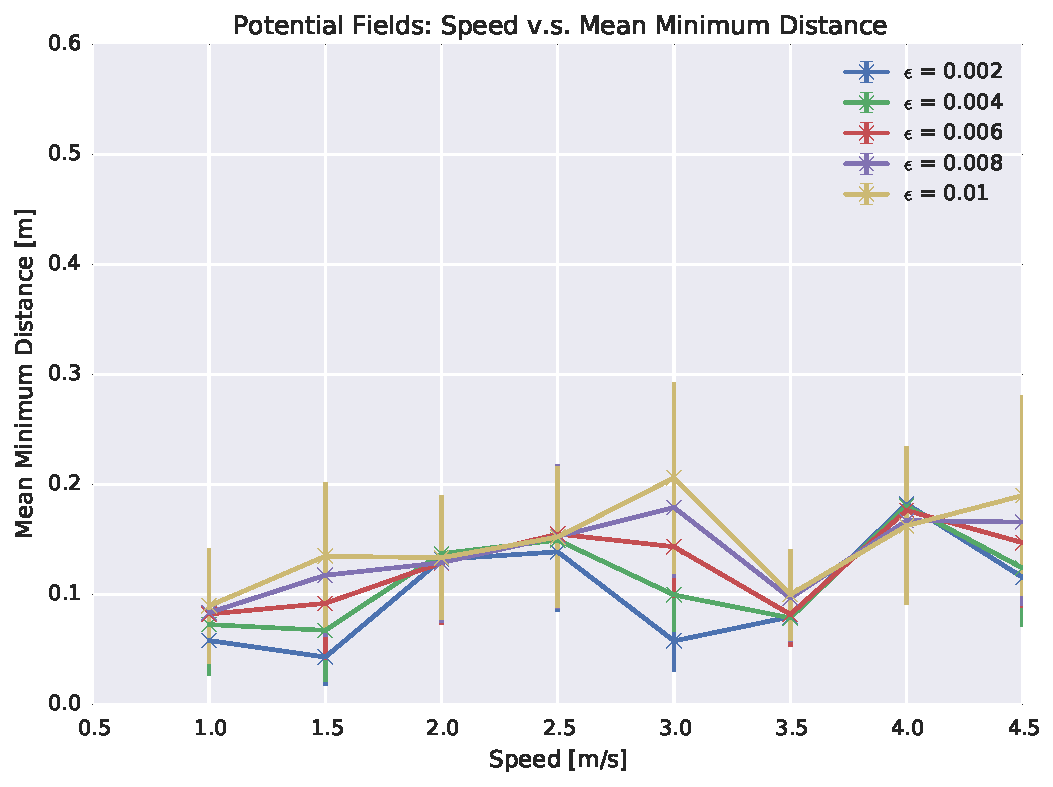
\includegraphics[width=0.48\linewidth]{figs/pf_mean_min_distance_0}

    \caption{Plots showing how the minimum distance to any obstacle for a path
        changes as the speed increases for various amounts of obstacle position
        uncertainties.  The horizontal axis represents the speed of the robot
        and the vertical axis represents the minimum distance to obstacles
        along the path. The different lines on each plot represent experiments
    with differing amounts of noise and the error bars represent one standard
deviation. On the left is the graph for Dodger and on the right is the graph
for the potential fields planner.}

    \label{fig:plot_min_distance}
\end{figure}

Fig.~\ref{fig:plot_max_cost} shows how the maximum cost experienced along a
path given by the cost distribution changes as a function of the set speed of
the robot. The smaller the maximum cost, the safer the path. The figures shows
that as the speed increases, the maximum cost experienced by a robot being
planned using Dodger decreased. This is because when the robot is able to move
faster, it can maneuver through areas that only have a low cost for a small
period of time before becoming high cost areas again. Also, as the speed
increased over 2 $m/s$, there was a greater difference between the maximum
costs for paths through experimental configurations with small amounts of noise
and the maximum costs for paths through high noise configurations.  This is due
to the fact that no matter how fast the robot is able to move, the more noise
in a scene, the more the initial path will not represent the actual costs
through the environment and the planner will need to replan. The robot may move
to an area in which it thinks it will be safe, but if the obstacles deviate
from their prescribed trajectories, this area may not be safe any longer and a
new path is needed and therefore the cost for the path a robot is executing
will increase.  The paths generated by the potential fields planner did not
have a similar behaviour as the amount of noise increased, however, the maximum
cost was greater for all speeds than that of the paths generated by Dodger.
This is because the potential fields planner does not take into account the
trajectories of the obstacles when planning and is purely reactive. This plot
shows that having access to information about where obstacles are moving can
decrease the costs of the generated paths which in turn leads to safer
trajectories for the robot.

\begin{figure}[h!]
    \centering
    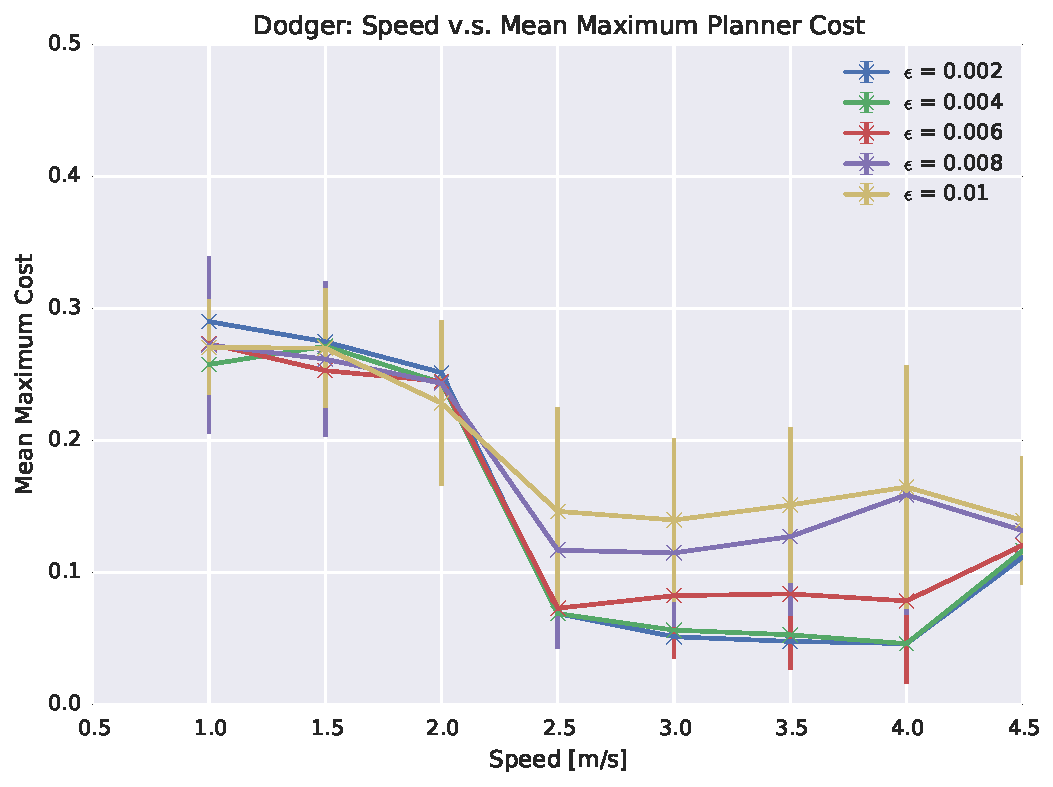
\includegraphics[width=0.48\linewidth]{figs/planner_mean_max_cost_0}
    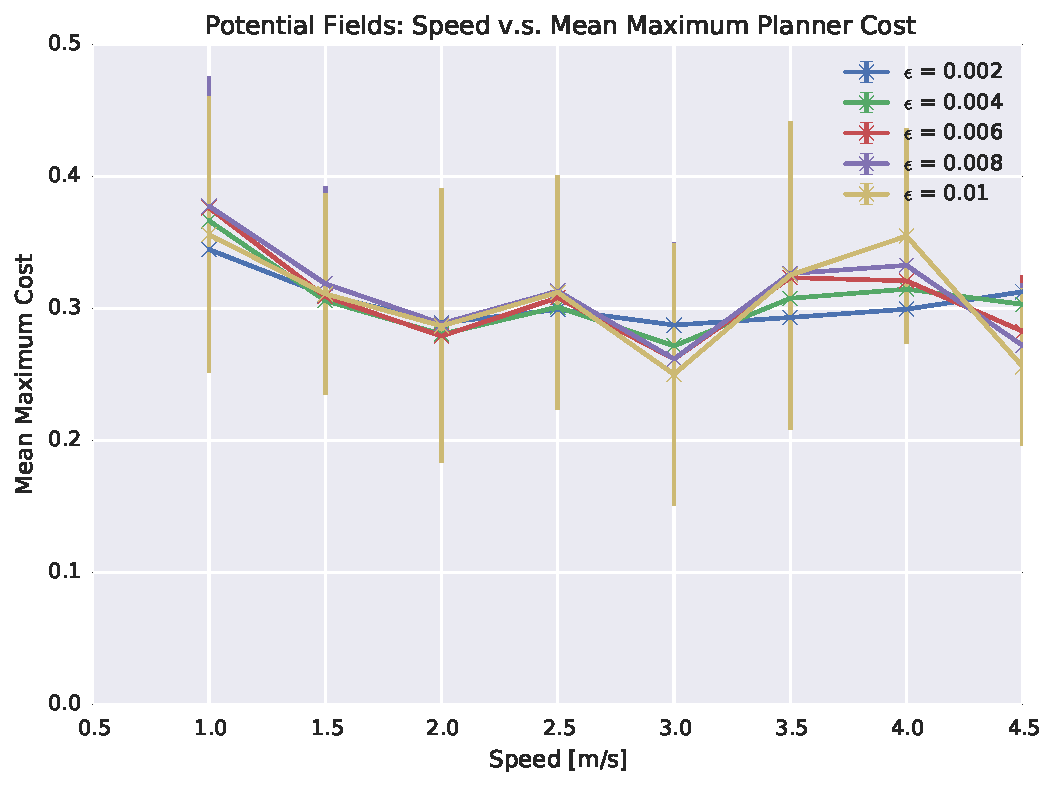
\includegraphics[width=0.48\linewidth]{figs/pf_mean_max_cost_0}

    \caption{Plots showing how the maximum cost for a path changes as the
        speed increases for various amounts of obstacle position uncertainties.
        The horizontal axis represents the speed of the robot and the vertical
        axis represents the maximum cost along the path. The different lines on
    each plot represent experiments with differing amounts of noise and the
error bars represent one standard deviation.  On the left is the graph for
Dodger and on the right is the graph for the potential fields planner.}

    \label{fig:plot_max_cost}
\end{figure}

Fig.~\ref{fig:plot_avg_cost} shows how the average cost along a path changes as
the speed of the robot increases for Dodger and the potential fields planner.
These plots are very similar to those in Fig.~\ref{fig:plot_max_cost} however,
there is an increase in the average cost for the potential fields. This is
mostly likely because as the speed of the robot increases, the potential fields
planner is able to move the robot through the path of an obstacle without being
deviated or hit by the obstacle thus increasing the average cost along the
path. Since the planner can move the robot through these areas quickly, instead
of planning around the obstacle, the planner will just move quickly through the
path of the obstacle. From these plots, it is evident that Dodger was able to
generate paths with lower average costs than potential fields and as the speed
of the robot increased, the average costs of the paths for Dodger decreased
whereas the costs for paths generated by potential fields increased.

\begin{figure}[h!]
    \centering
    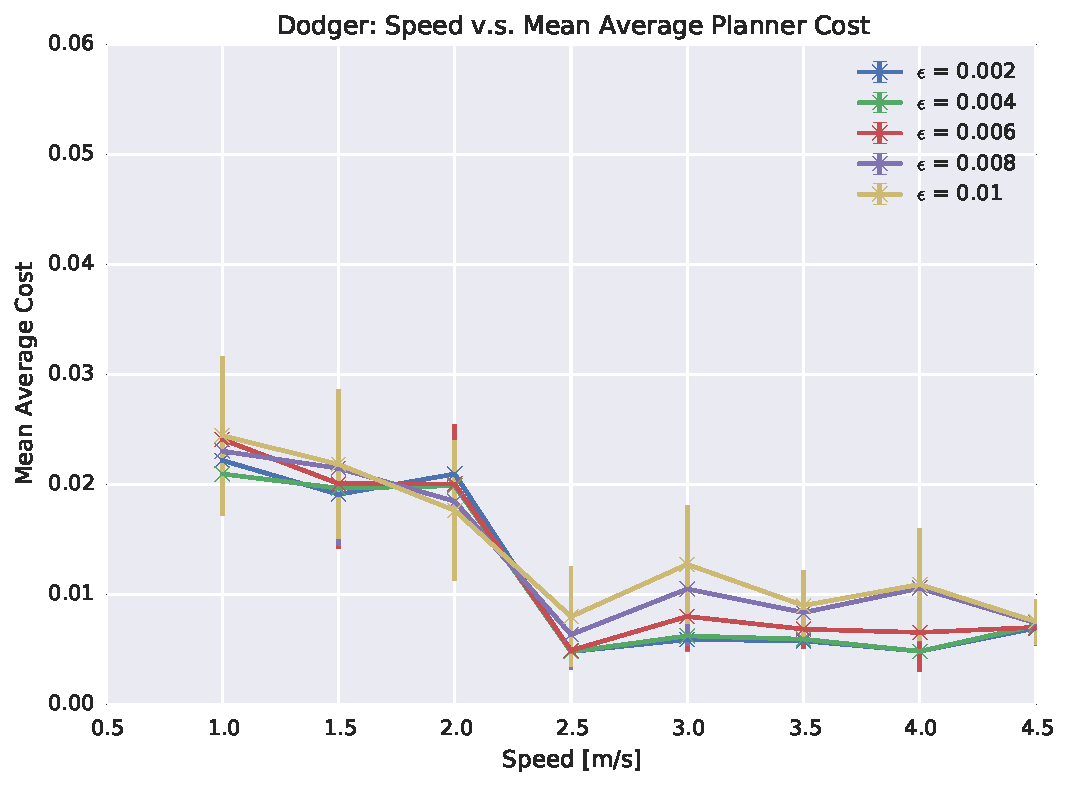
\includegraphics[width=0.48\linewidth]{figs/planner_mean_avg_cost_0}
    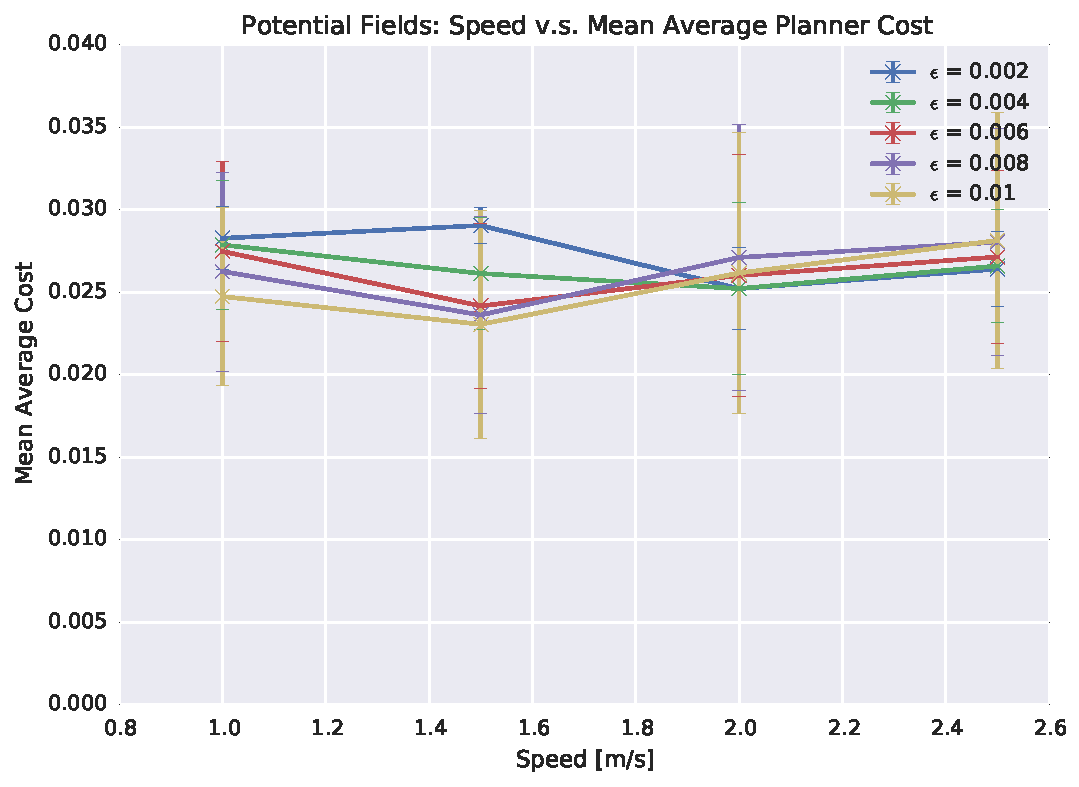
\includegraphics[width=0.48\linewidth]{figs/pf_mean_avg_cost_0}

    \caption{Plots showing how the average cost for a path changes as the
        speed increases for various amounts of obstacle position uncertainties.
        The horizontal axis represents the speed of the robot and the vertical
        axis represents the average cost along the path. The different lines on
    each plot represent experiments with differing amounts of noise and the
error bars represent one standard deviation.  On the left is the graph for
Dodger and on the right is the graph for the potential fields planner.}

    \label{fig:plot_avg_cost}
\end{figure}

\subsection{Variance}

Representing the standard deviation as a function of the noise quantifies how
consistent the planner is as the noise for a scene changes.The plots in
Fig.~\ref{fig:plot_std_min_distance} show how the standard deviation for the
minimum distance metrics increases as the noise injected into the obstacle
trajectory increases and the speed changes. The standard deviation for minimum
distance metric increased more rapidly for Dodger than for the potential fields
planner.  This is because there is a stochastic component in the planning for
Dodger, the probabilistic roadmap. For some random generations of the roadmap,
areas around where the obstacles are going to be are more heavily sampled, thus
leading to greater variance in the results for the minimum distance. For the
potential fields planner, there is no random component and is free to sample
along the execution of its path and thus the standard deviation for this metric
is only determined by the stochasticity of the dynamic obstacles and not by the
algorithm.

\begin{figure}[h!]
    \centering
    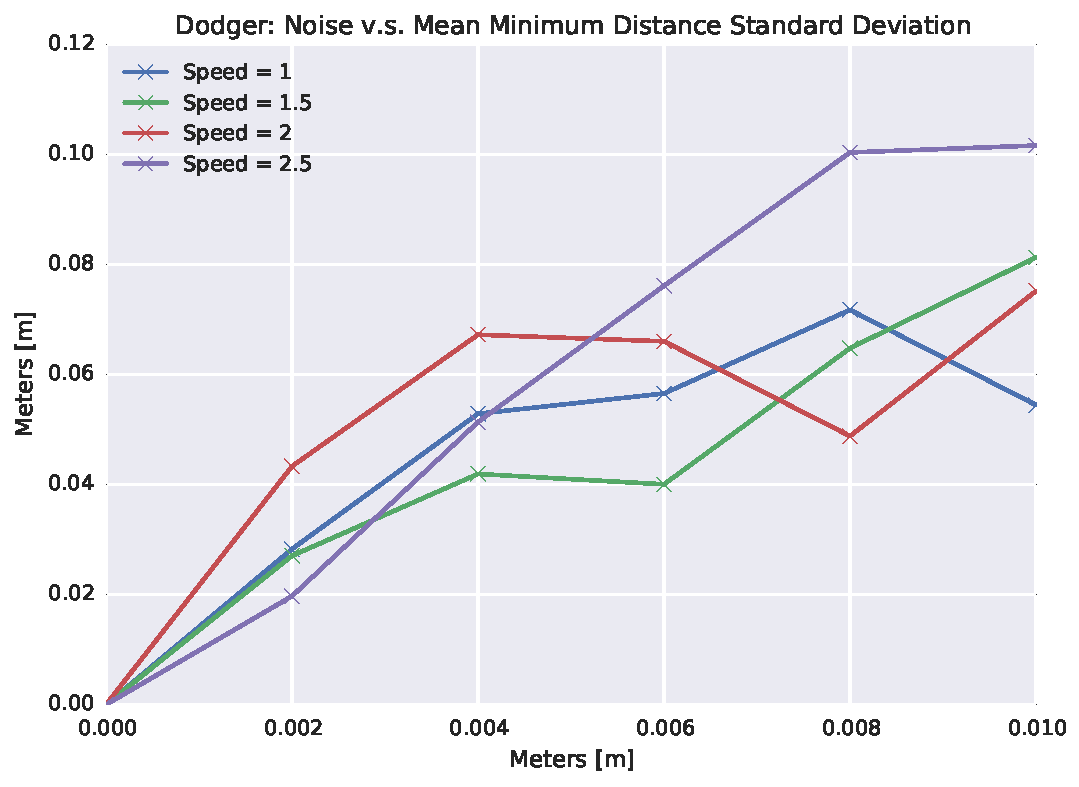
\includegraphics[width=0.48\linewidth]{figs/planner_std_min_distance_0}
    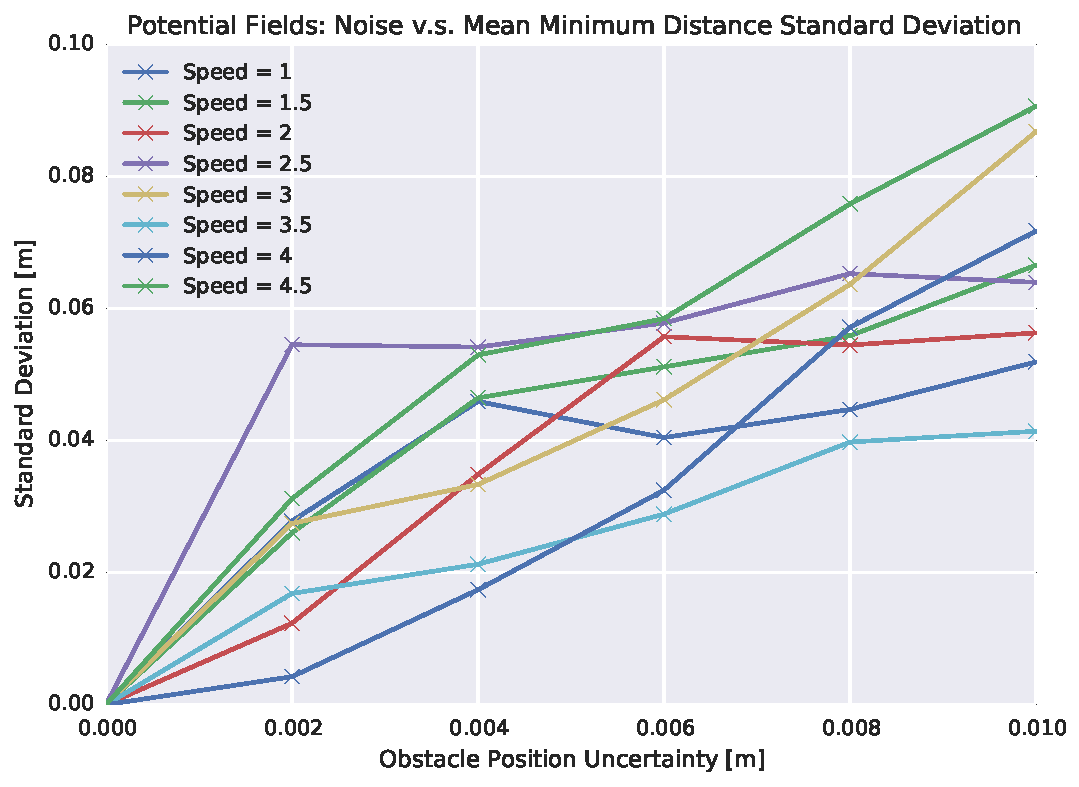
\includegraphics[width=0.48\linewidth]{figs/pf_std_min_distance_0}

    \caption{Plots showing how the standard deviation for the minimum distance
        along a path changes as the noise injected into the obstacle
        trajectories increases. The horizontal axis represents the amount of
        noise and the vertical axis represents the standard deviation. The
        different lines indicate different speeds that the robot was
    travelling. On the left is the graph for Dodger and on the right is the
graph for the potential fields planner.}

    \label{fig:plot_std_min_distance}
\end{figure}

The plots in Fig.~\ref{fig:plot_std_cost} shows how the average and maximum
costs change as the noise injected into the obstacle trajectories increases.
The average and minimum costs for the paths generated by Dodger increases less
rapidly than those generated by the potential fields planner. This is because
Dodger is actively searching for low cost paths through the environment using
the information about obstacle motion whereas the potential fields planner is
just reacting the change in the potentials leading to the goal. Since the
potential fields planner is not trying to minimize the cost of the generated
path, there will be a larger variance in the average and maximum costs.

\begin{figure}[h!]
    \centering
    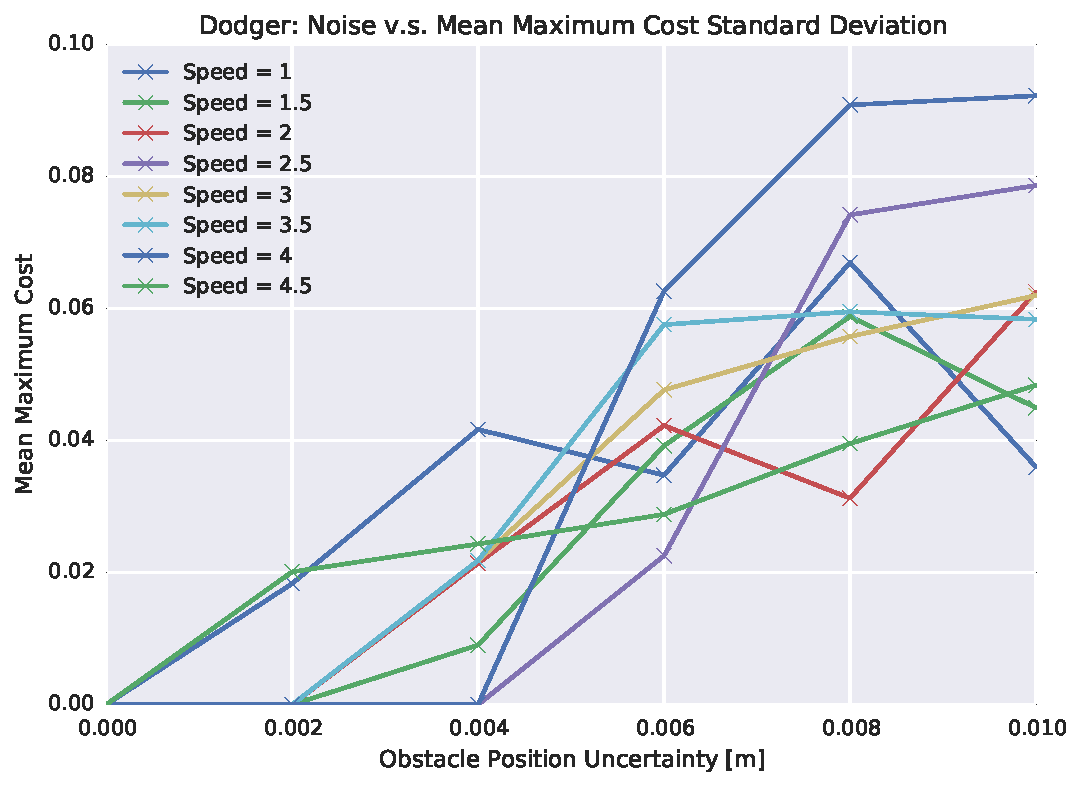
\includegraphics[width=0.48\linewidth]{figs/planner_std_max_cost_0}
    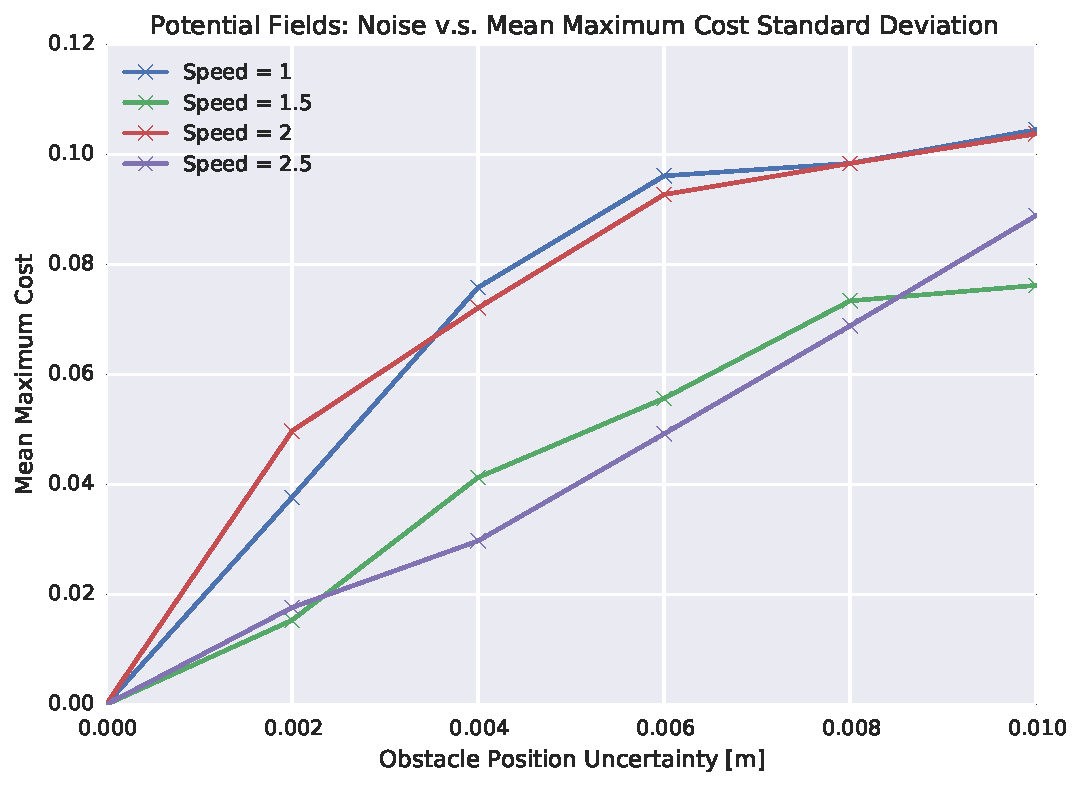
\includegraphics[width=0.48\linewidth]{figs/pf_std_max_cost_0} \\
    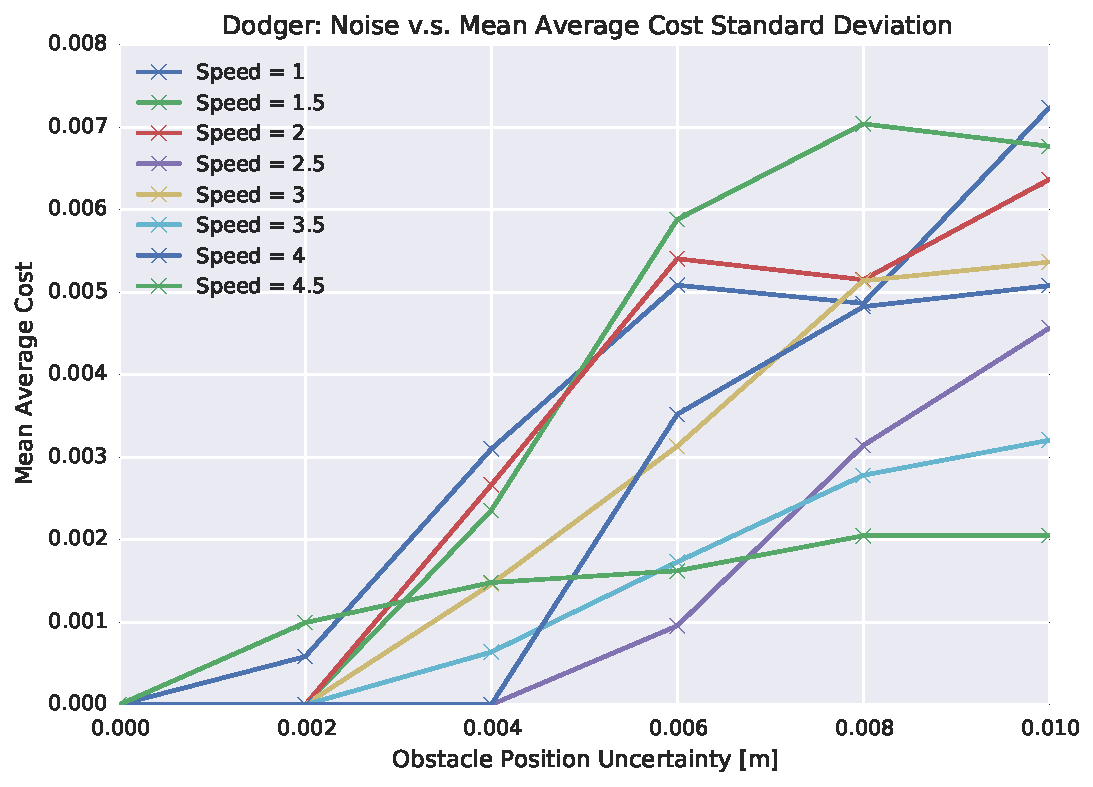
\includegraphics[width=0.48\linewidth]{figs/planner_std_avg_cost_0}
    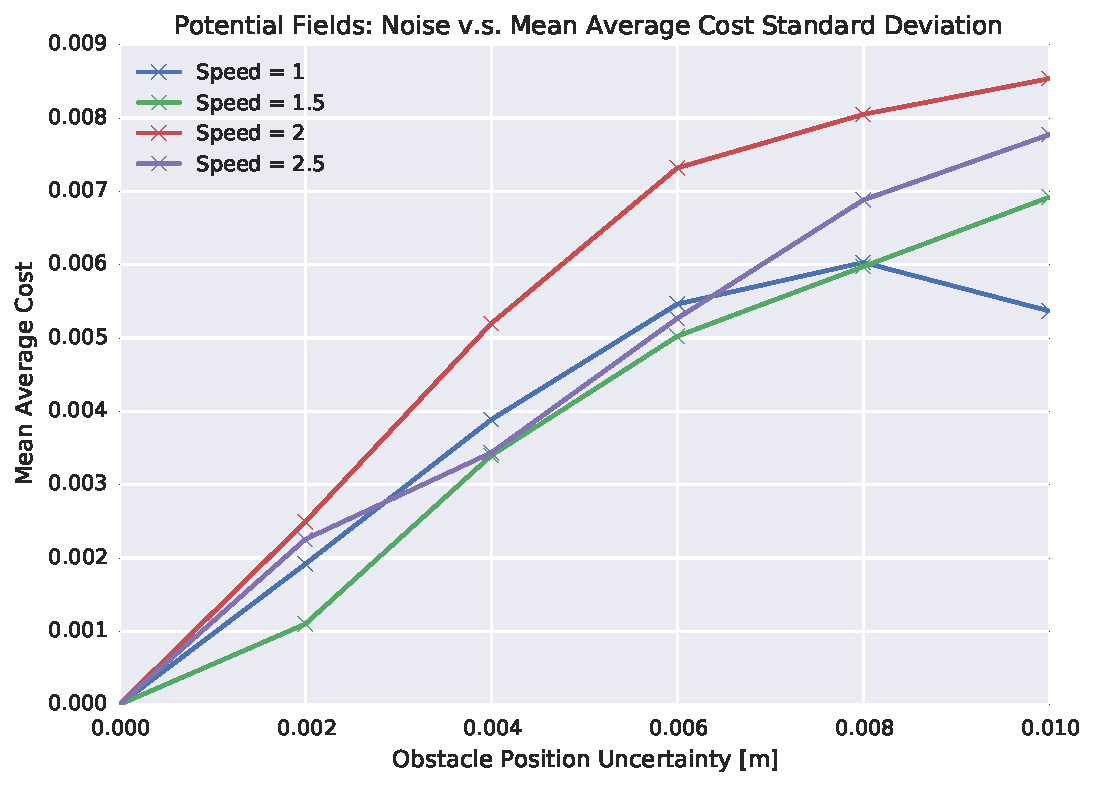
\includegraphics[width=0.48\linewidth]{figs/pf_std_avg_cost_0}

    \caption{Plots showing how the standard deviation for the maximum cost and
        average cost along a path changes as the noise injected into the
        obstacle trajectories increases. The horizontal axis represents the
        amount of noise and the vertical axis represents the standard
        deviation. The different lines indicate different speeds that the robot
        was travelling. On the left is the graph for Dodger and on the right is
    the graph for the potential fields planner. The top row is for the maximum
cost and the bottom row is the for the average cost.}

    \label{fig:plot_std_cost}
\end{figure}

\section{Computational Time}

Showing how the computational time changes for different sets of parameters is
useful to show how feasible the approach is in practice. For the two planners,
the times it took to compute the paths were collected and are shown in
Fig.~\ref{fig:plot_comp_time}. The potential fields planner is able to find
paths more quickly than Dodger and this is due to its purely reactive
behaviour.  Since the scenes used did not have any local minimas besides the
goal, the potential fields planner is able to quickly find a path to the goal
and as the speed increases, the amount of steps needed for it to search through
the environment decreases thus decreasing the overall computational time.  The
computational time for Dodger also decreased as the speed increased, but the
overall computational time was greater than potential fields. This is because
Dodger uses a much more complex algorithm than potential fields requiring more
computational time. For speeds less than 2.5 $m/s$, the time it takes Dodger to
find a path may be infeasible for some situations.  However, for speeds of 2.5
$m/s$, the computational time decreasing drastically making it feasible to use
for real-time scenarios.  Please note that computational times shown in
Fig.~\ref{fig:plot_comp_time} represent the overall time it takes the planner
to find a path with replanning.  This means that the planner is simultaneously
executing and planning thus meaning that the robot reached the goal in at least
the time presented in the figures.

\begin{figure}[h!]
    \centering
    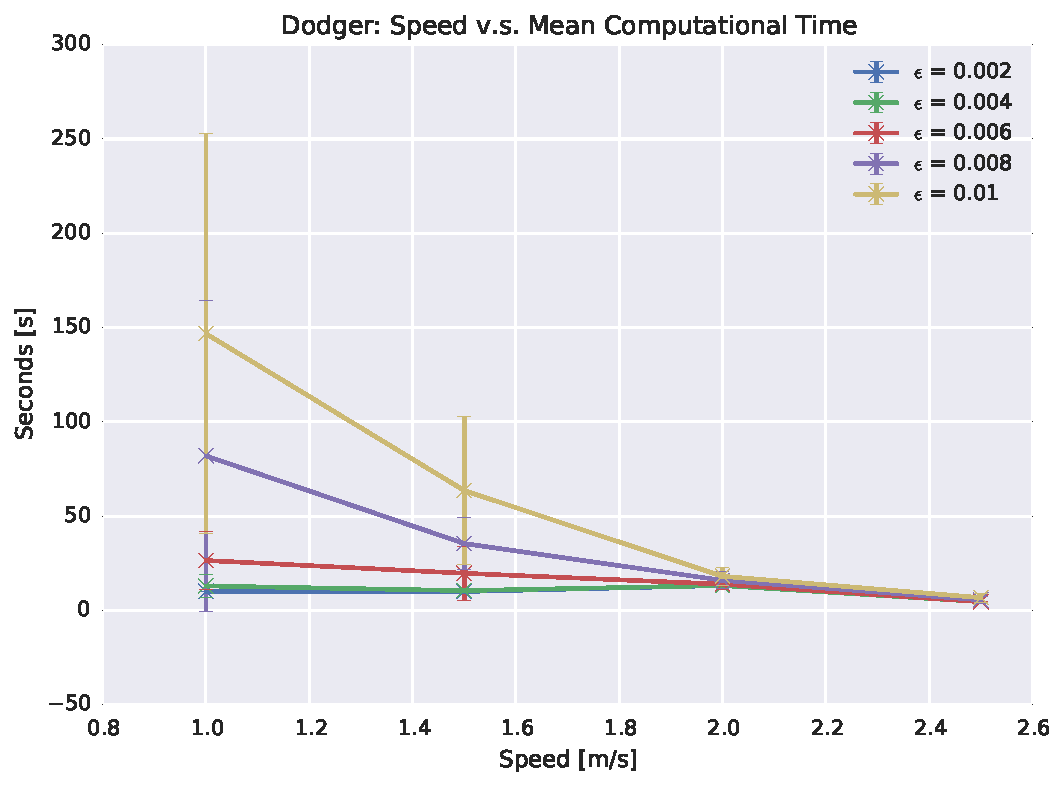
\includegraphics[width=0.48\linewidth]{figs/planner_mean_times_0}
    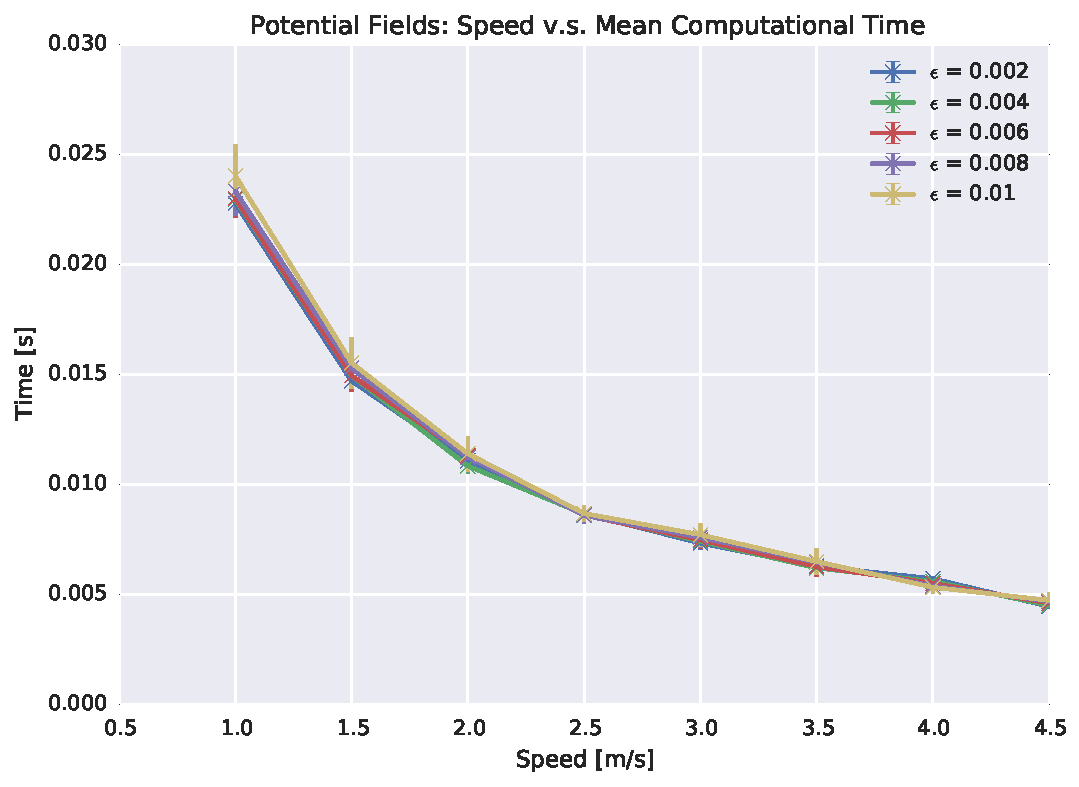
\includegraphics[width=0.48\linewidth]{figs/pf_mean_times_0} \\
    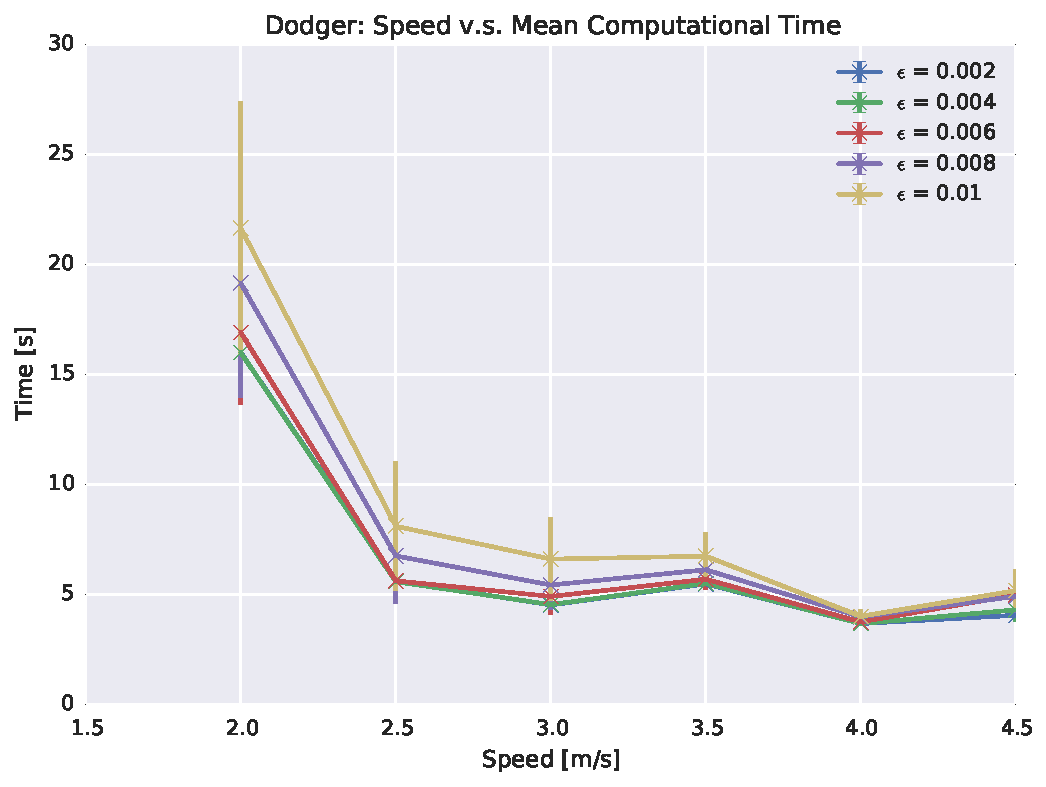
\includegraphics[width=0.48\linewidth]{figs/planner_small_mean_times_0}
    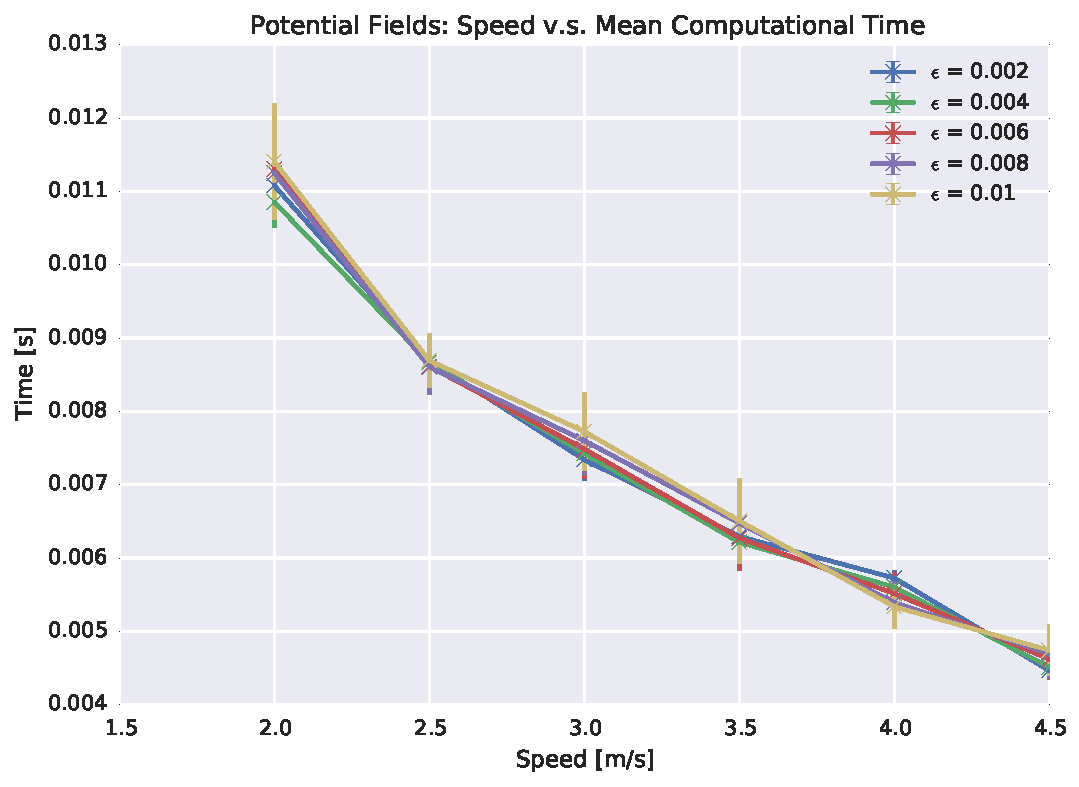
\includegraphics[width=0.48\linewidth]{figs/pf_small_mean_times_0}

    \caption{Plots showing how the computational to generate a path changes as
        the speed increases for various amounts of obstacle position
        uncertainties.  The horizontal axis represents the speed of the robot
        and the vertical axis represents the computational time to generate the
        path. The different lines on each plot represent experiments with
        differing amounts of noise and the error bars represent one standard
        deviation.  On the left is the graph for Dodger and on the right is the
    graph for the potential fields planner.}

    \label{fig:plot_comp_time}
\end{figure}

\subsection{Variance}

As with the other metrics, seeing how the variance reacts to an increasing
amount of noise is equally as important. Fig.~\ref{fig:plot_std_comp_time}
presents this relationship. The standard deviations for computational times for
Dodger increase more rapidly than for the potential fields planner. This is
because the Dodger had significantly larger computational times than the
potential fields planner and would also have higher standard deviations.
Likewise, the computational time standard deviations for Dodger are caused by
both the randomness of the nodes used to create the probabilistic roadmap and
the level of uncertainty injected into the obstacle trajectories. The standard
deviation for the computational times for the potential fields planner is only
dependent on the amount of noise in the obstacles movements since the algorithm
does not have any random components.

\begin{figure}[h!]
    \centering
    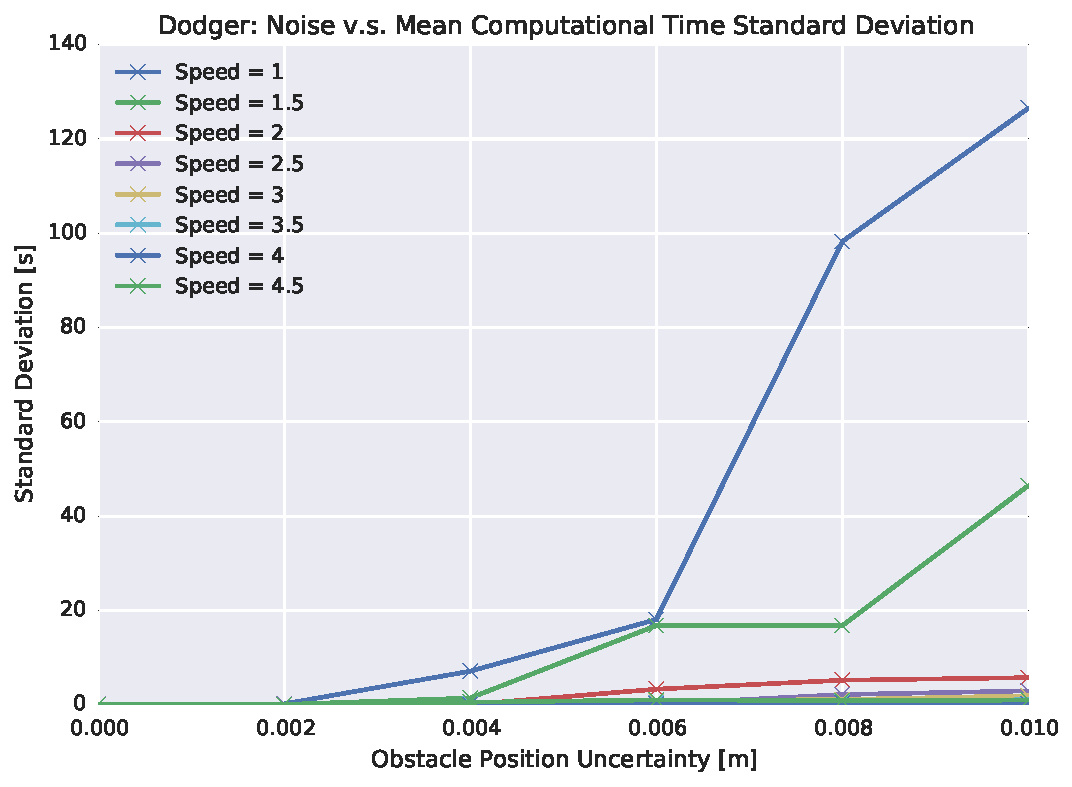
\includegraphics[width=0.48\linewidth]{figs/planner_std_avg_times_0}
    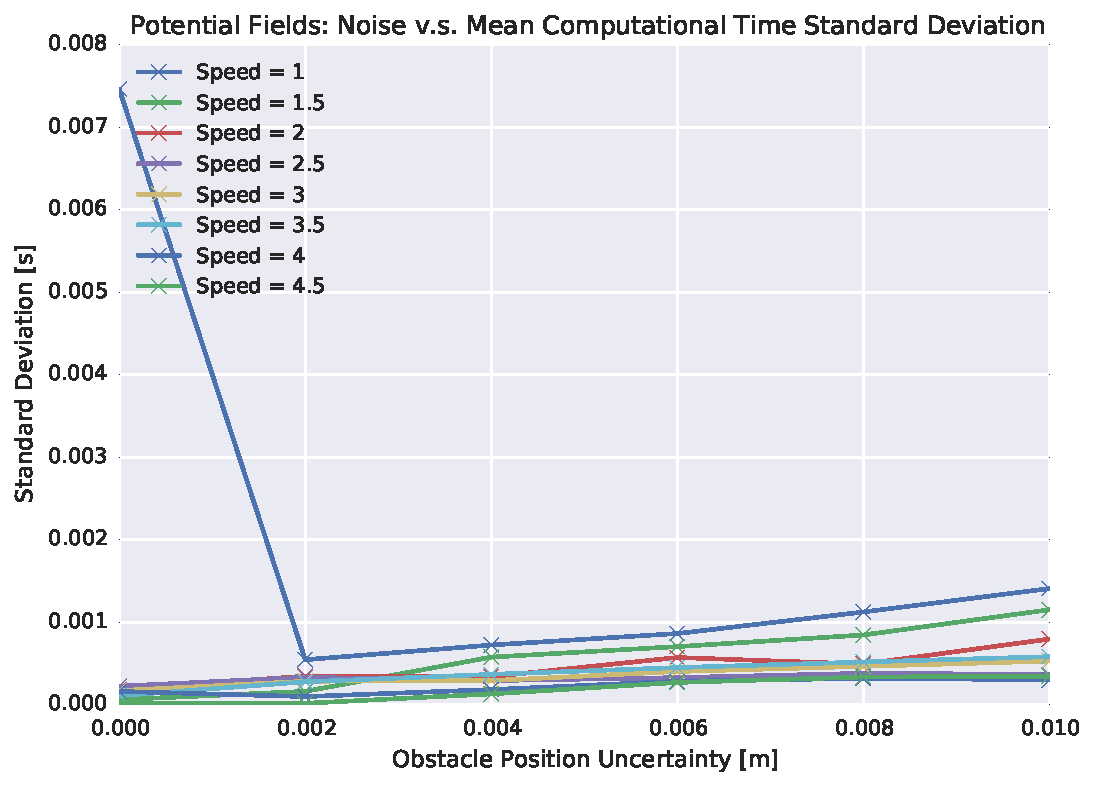
\includegraphics[width=0.48\linewidth]{figs/pf_std_avg_times_0}

    \caption{Plots showing how the standard deviation for the computational
        cost to generate a path changes as the noise injected into the obstacle
        trajectories increases.  The horizontal axis represents the amount of
        noise and the vertical axis represents the standard deviation. The
    different lines indicate different speeds that the robot was travelling. On
the left is the graph for Dodger and on the right is the graph for the
potential fields planner.}

    \label{fig:plot_std_comp_time}
\end{figure}

\section{Behaviour}

Figures~\ref{fig:dodger} and~\ref{fig:pf} show how Dodger and the potential
fields planner respectively guide the robot through Scene 1 when the noise
injected into the obstacle trajectories, $\epsilon = 0.004$ and the speed, $s =
1.5 m/s$. The robot is represented by the quadrotor, its path by the blue line,
the obstacles by the mobile ground robots, and the initial and goal
configurations by the red and green quadrotors respectively. Qualitatively, the
paths generated by Dodger look safer than that of those generated by the
potential fields planner.  The potential fields planner even led the robot into
collisions twice in the third and sixth snapshots in Fig.~\ref{fig:pf}. This is
because the obstacles are not within the sensing radius of the robot using
potential fields until they are at their maximum velocity in the center of the
scene and the robot is not able to move out of their way. Dodger generates a
path that automatically moves the robot around the back of the oscillating
obstacles such that it does not cross over their trajectories from side to
side. This reduces the cost associated with the path and significantly reduces
the chance that the robot will collide with an obstacle. Due to the
stochasticity of the obstacles' movements, Dodger needed to replan more than
once when executing the initial path. This occurred right before images three,
four, and six. The path becomes jagged and changes direction quickly. This is
because the original path is no longer safe because of the random movement of
the obstacles.

\begin{figure}[h!]
    \centering
    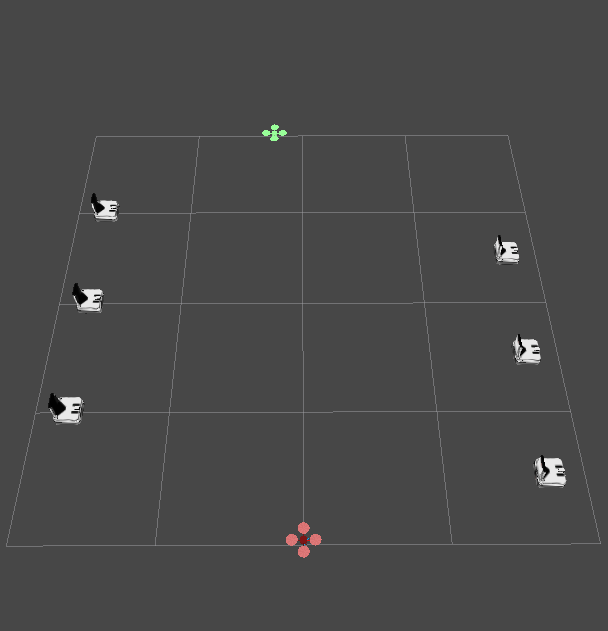
\includegraphics[width=0.32\linewidth]{figs/dodger_0}
    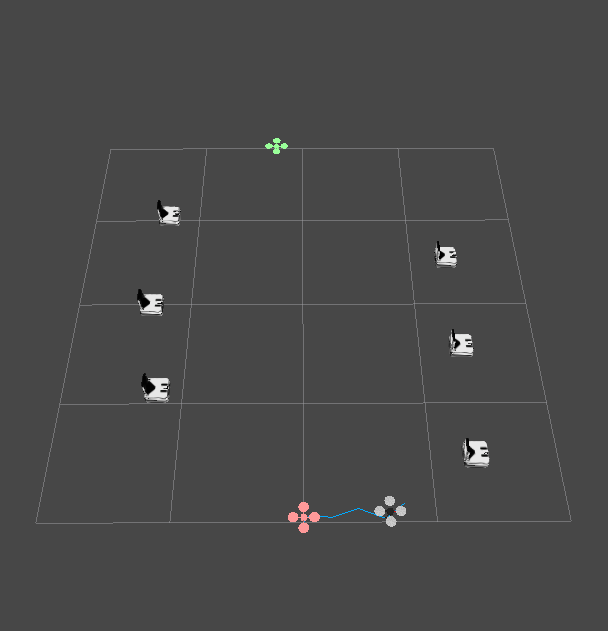
\includegraphics[width=0.32\linewidth]{figs/dodger_1}
    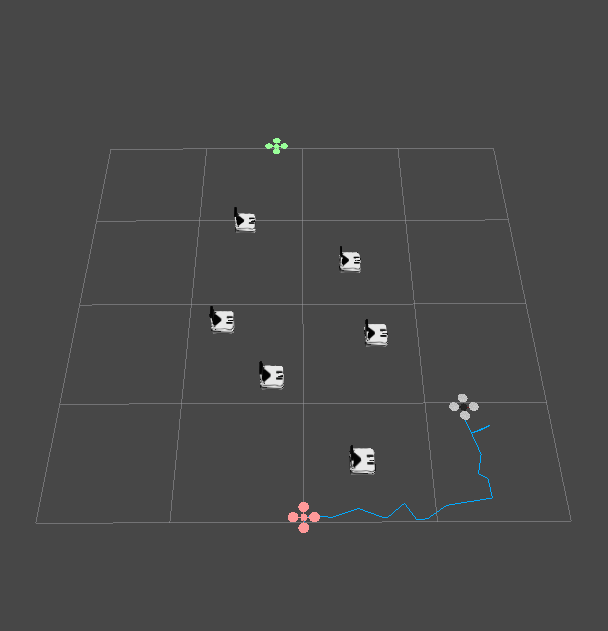
\includegraphics[width=0.32\linewidth]{figs/dodger_4} \\
    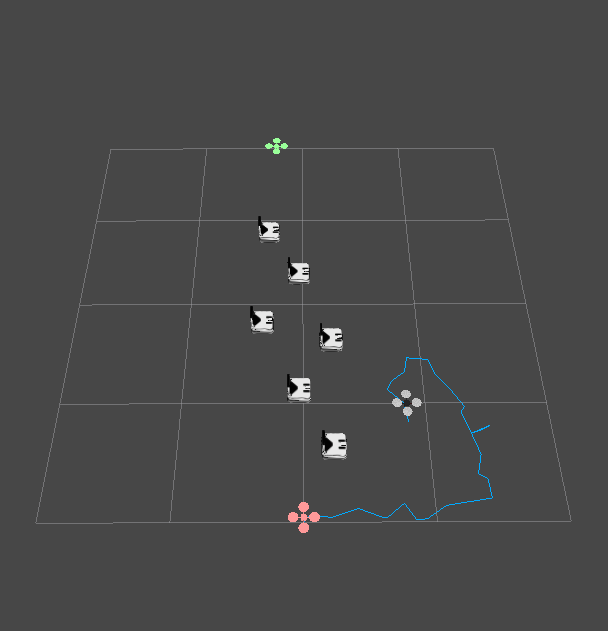
\includegraphics[width=0.32\linewidth]{figs/dodger_6}
    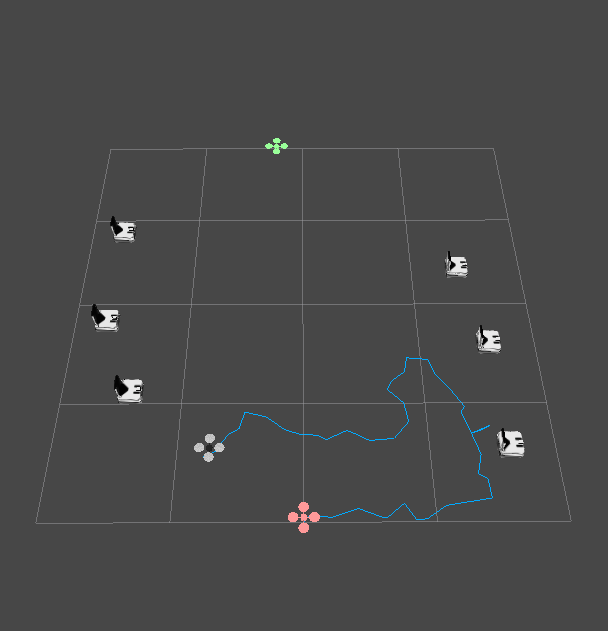
\includegraphics[width=0.32\linewidth]{figs/dodger_9}
    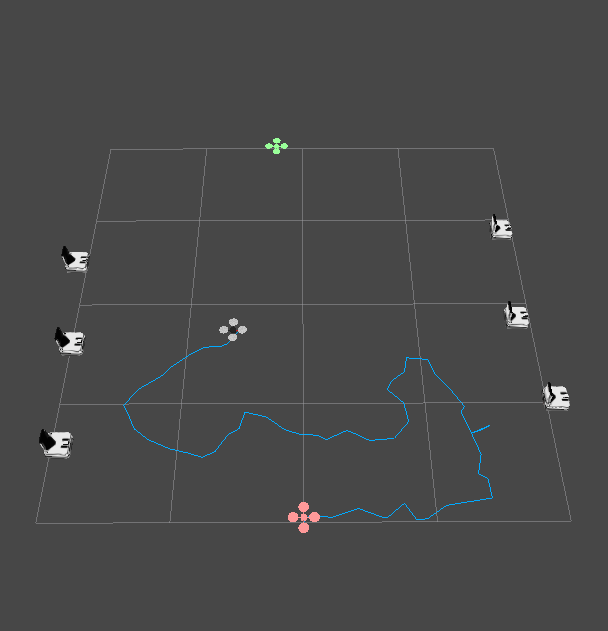
\includegraphics[width=0.32\linewidth]{figs/dodger_12} \\
    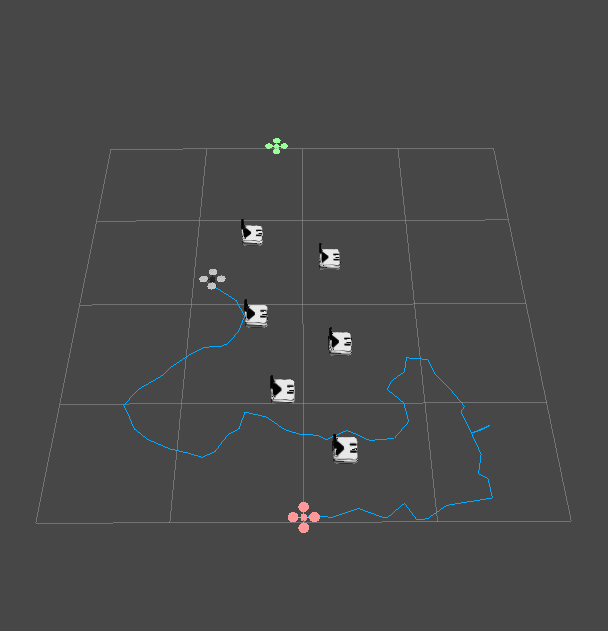
\includegraphics[width=0.32\linewidth]{figs/dodger_13}
    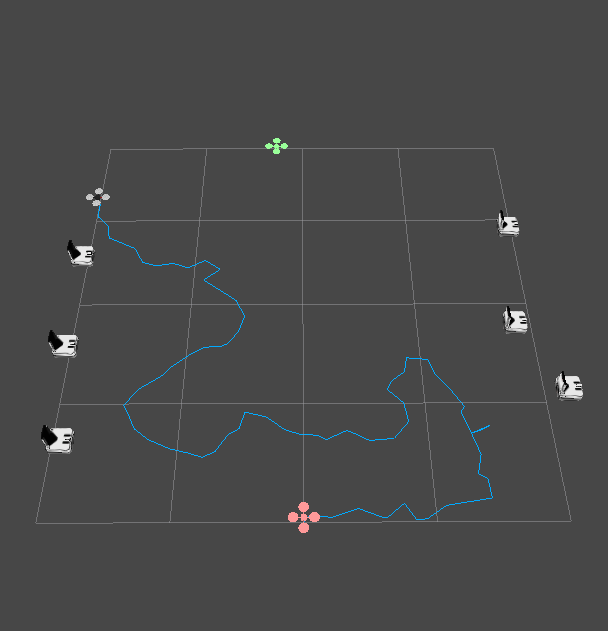
\includegraphics[width=0.32\linewidth]{figs/dodger_16}
    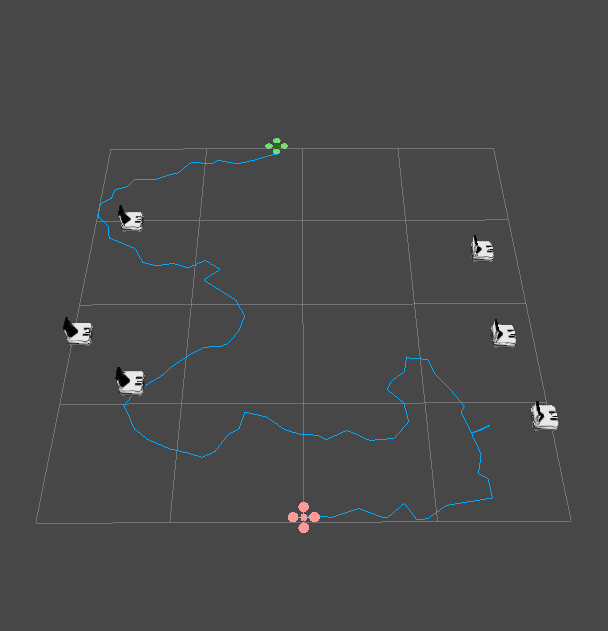
\includegraphics[width=0.32\linewidth]{figs/dodger_19}

    \caption{Images showing the progression of the robot, represented by the
    quadrotor, following a path generated by Dodger through Scene 1 from the
initial configuration, represented by the red quadrotor shape, to the goal
configuration, the green quadrotor shape.  The obstacles are represented by the
mobile ground robots and the path of the robot is shown by the blue line. The
sequence of images progress from left to right, up to down.}

    \label{fig:dodger}
\end{figure}

\begin{figure}[h!]
    \centering
    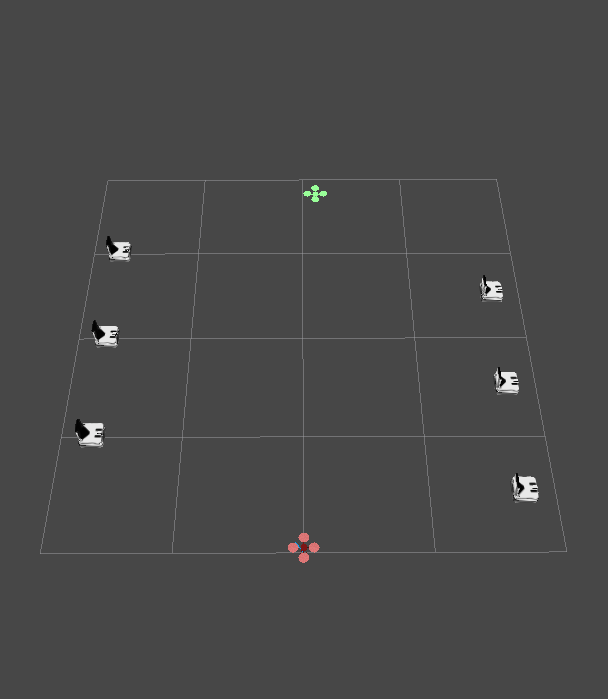
\includegraphics[width=0.32\linewidth]{figs/pf_0}
    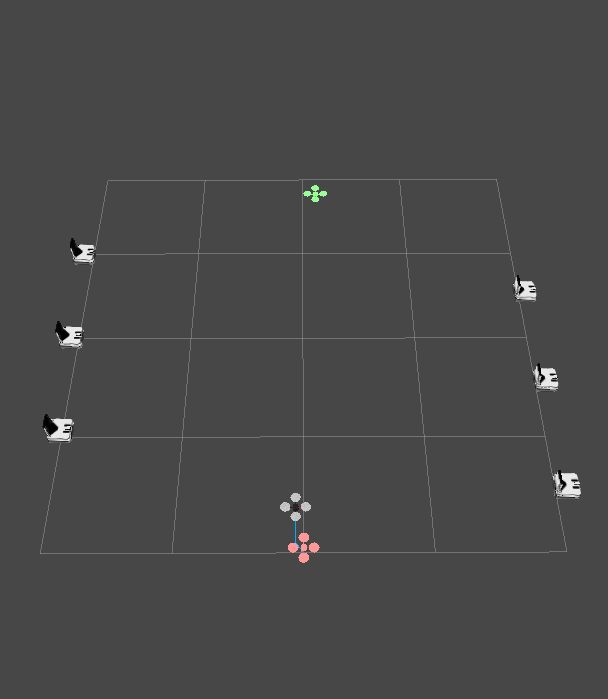
\includegraphics[width=0.32\linewidth]{figs/pf_1}
    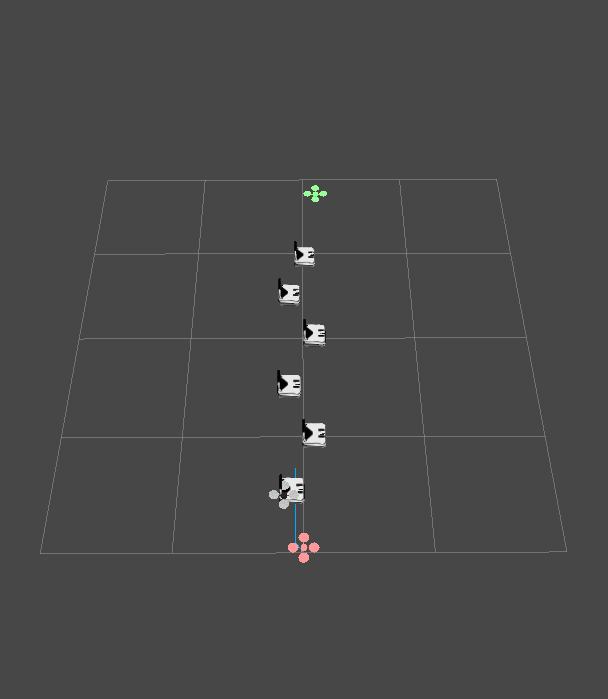
\includegraphics[width=0.32\linewidth]{figs/pf_3} \\
    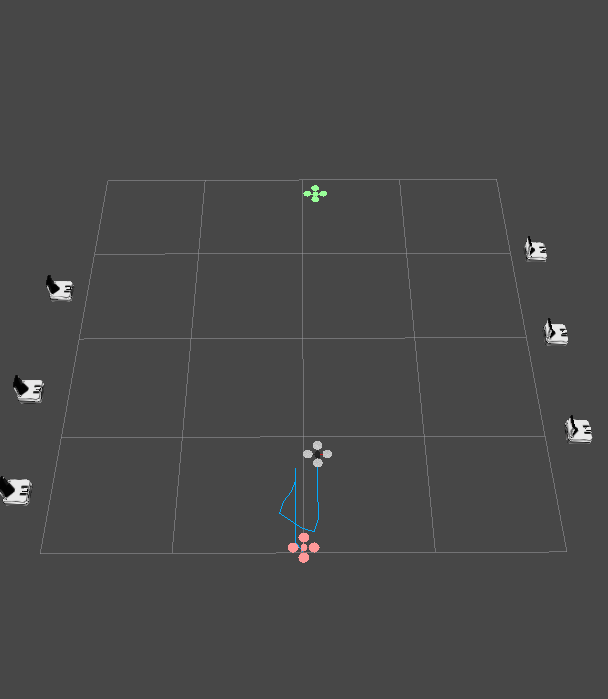
\includegraphics[width=0.32\linewidth]{figs/pf_6}
    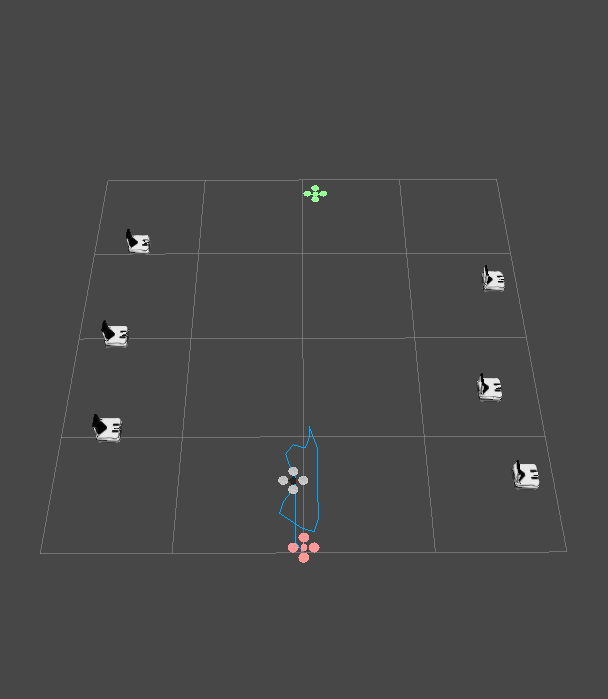
\includegraphics[width=0.32\linewidth]{figs/pf_9}
    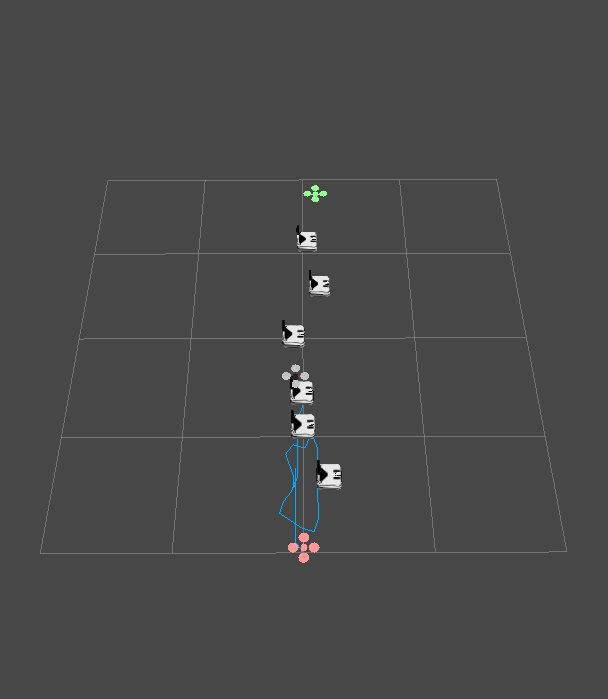
\includegraphics[width=0.32\linewidth]{figs/pf_12} \\
    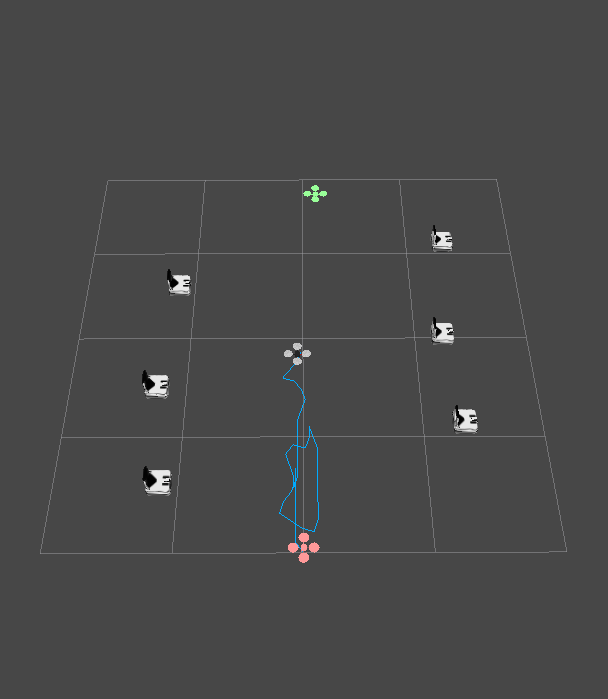
\includegraphics[width=0.32\linewidth]{figs/pf_13}
    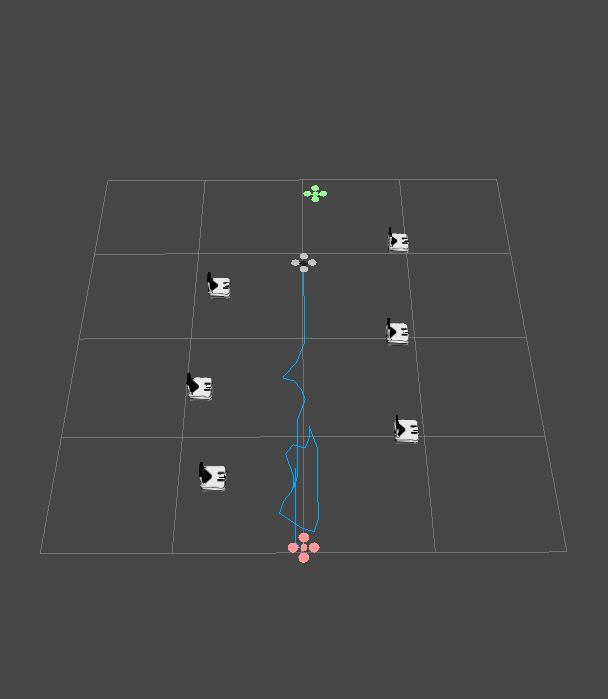
\includegraphics[width=0.32\linewidth]{figs/pf_16}
    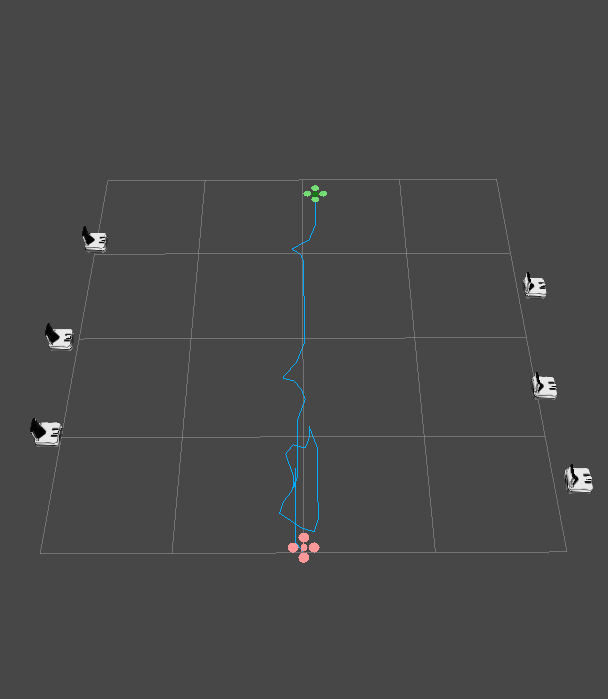
\includegraphics[width=0.32\linewidth]{figs/pf_19}

    \caption{Images showing the progression of the robot, represented by the
    quadrotor, following a path generated by the potential fields planner
    through Scene 1 from the initial configuration, represented by the red
    quadrotor shape, to the goal configuration, the green quadrotor shape.  The
    obstacles are represented by the mobile ground robots and the path of the
robot is shown by the blue line. The sequence of images progress from left to
right, up to down.}

    \label{fig:pf}
\end{figure}


\end{document}
